\scanpage{95}
% archive sheet number: 97

structures réelles s'identifie à $G^-$, qui est un \uline{torseur} sous $G^+$ par translation à gauche. Par contre, l'opération de $G^+$ sur $G^-$ par autom intérieurs n'est pas libre, le centre $Z=\{\pm1\}$ de $G$ opère trivialement, et il y a deux orbites sous $G^+$ (ou mieux $G^+/Z$)

\deleted{Donc on trouve} les $2$ \unsure{st|et} \inserted{(pour $n=4$ ou $6$)} les symétries par rapp. respectivement aux sommets et aux arêtes des \deleted{\unsure{ca|co}} polygones (carré ou hexagone) \unsure{fondamentaux|fondamental}.

\figure{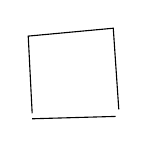
\begin{tikzpicture}[x=1cm,y=1cm]\draw (0,0.05) -- (-0.05,1.03) -- (1.03,1.13) -- (1.10,0.10);\draw (0,-0.02) -- (1.06,0.01);\end{tikzpicture}}

\uline{Donc} on résume

\uline{Proposition}. Soit une courbe elliptique \deleted{réelle} complexe. \deleted{Pour qu'elle admette une} Les structures réelles \inserted{sur $X$} \deleted{\unsure{qu'il s|i.e.}} \deleted{qu'elle} correspondent aux \inserted{anti} autom \deleted{\unsure{involutifs|involutif}} de la courbe \inserted{elliptique} conforme \deleted{positive ?} \deleted{qu'il y en a} et il y en a si et seulement si la suite

\diagram{\begin{tikzcd}[ampersand replacement=\&,column sep=small]
1\arrow[r,dash]\&G^+\arrow[r,dash]\&G\arrow[r,dash]\&\pm1,\arrow[r,dash]\&\unsure{1|\phi}
\end{tikzcd}}

est exacte (à droite). Dans ce cas, $G$ est \inserted{isom au} \deleted{au} groupe diédral \inserted{$D_n$} dont $G^+$ (d'ordre \inserted{$n=$}$2,4$ ou $6$) est le groupe des rotations. L'ens des structures réelles se partage en deux orbites sous $G^+$, (opérant par autom intérieurs), et les structures réelles correspondant à deux orbites distinctes sont (par définition !) non isomorphes. \deleted{et les deux orbites correspondent aux structures $E_a,E'_a$}

Je présume que si l'une est formé de structures $E_a$ ($a\in\mathbb R^{*+}$ fixé), l'autre est formé des structures $E'_a$ (avec le $=$ $a$), et inversement, i.e. qu'on peut trouver un $a\in\mathbb R^{*+}$ unique, tel que les deux orbites sont l'une formée des structures isom à $E_a$, l'autre des structures isom à $E'_a$. De plus il faudrait.
